\setcounter{section}{16}


\section{Lecture 17: Feb 26}


\subsection*{Last time}
\begin{itemize}
 \item Unusual and influential data (JF chapter 11)
\end{itemize}


\subsection*{Today}
\begin{itemize}
 \item Added-variable plots
 \item Should unusual data be discarded
\end{itemize}



\subsection*{Added-variable plots}
Unlike the case of SLR, the scatterplot with the response variable and one predictor gives only the marginal effect in MLR.
Instead, the \underline{added-variable plot} (also called a partial-regression plot or a partial-regression leverage plot) gives a graphical inspection over each dimension.

Let $\hat{Y}_i^{(1)}$ represent the residuals from the least-squares regression of $Y$ on all the $X$s except $X_1$, in other words, the residuals from the following fitted regression equation:
$$
Y_i = \tilde{\beta}_0 ^{(1)} +  \tilde{\beta}_2^{(1)} X_{i2} + \dots +  \tilde{\beta}_p ^{(1)} X_{ip} + \tilde{Y}_i^{(1)}
$$  
where the parenthetical superscript $(1)$ indicates the omission of $X_1$ from the right-hand side of the regression equation.
Likewise, $X_i^{(1)}$ is the residual from the least-squares regression of $X_1$ on all the other $X$s:
$$
X_{i1} = \check{\beta}_0^{(1)} +  \check{\beta}_2^{(1)} X_{i2} + \dots +  \check{\beta}_p^{(1)} X_{ip} + \check{X}_i^{(1)}
$$
Then, the residuals $ \tilde{Y}_i^{(1)}$ and $\check{X}_i^{(1)}$ have the following interesting properties:
\begin{enumerate}
  \item The slope from the least-squares regression of  $ \tilde{Y}_i^{(1)}$ on $\check{X}_i^{(1)}$ is simply the least-squares slope $\hat{\beta}_1$ from the {\it full} multiple regression.
  \item The residuals from the simple regression of $ \tilde{Y}_i^{(1)}$ on $\check{X}_i^{(1)}$ are the same as those from the full regression, that is
  $$
 \tilde{Y}_i^{(1)} = \hat{\beta}_1 \check{X}_i^{(1)} + \hat{\epsilon}_i
  $$
  \item The variation of $\check{X}_i^{(1)}$ is the {\it conditional variation} of $X_1$ holding the other $X$s constant.
\end{enumerate}

Figure~\ref{fig:avp} shows that the conditional variation is smaller than its marginal variation -- much smaller  when $X_1$ is strongly collinear with other $X$s, 
%
\begin{figure}[H]
\begin{center}
  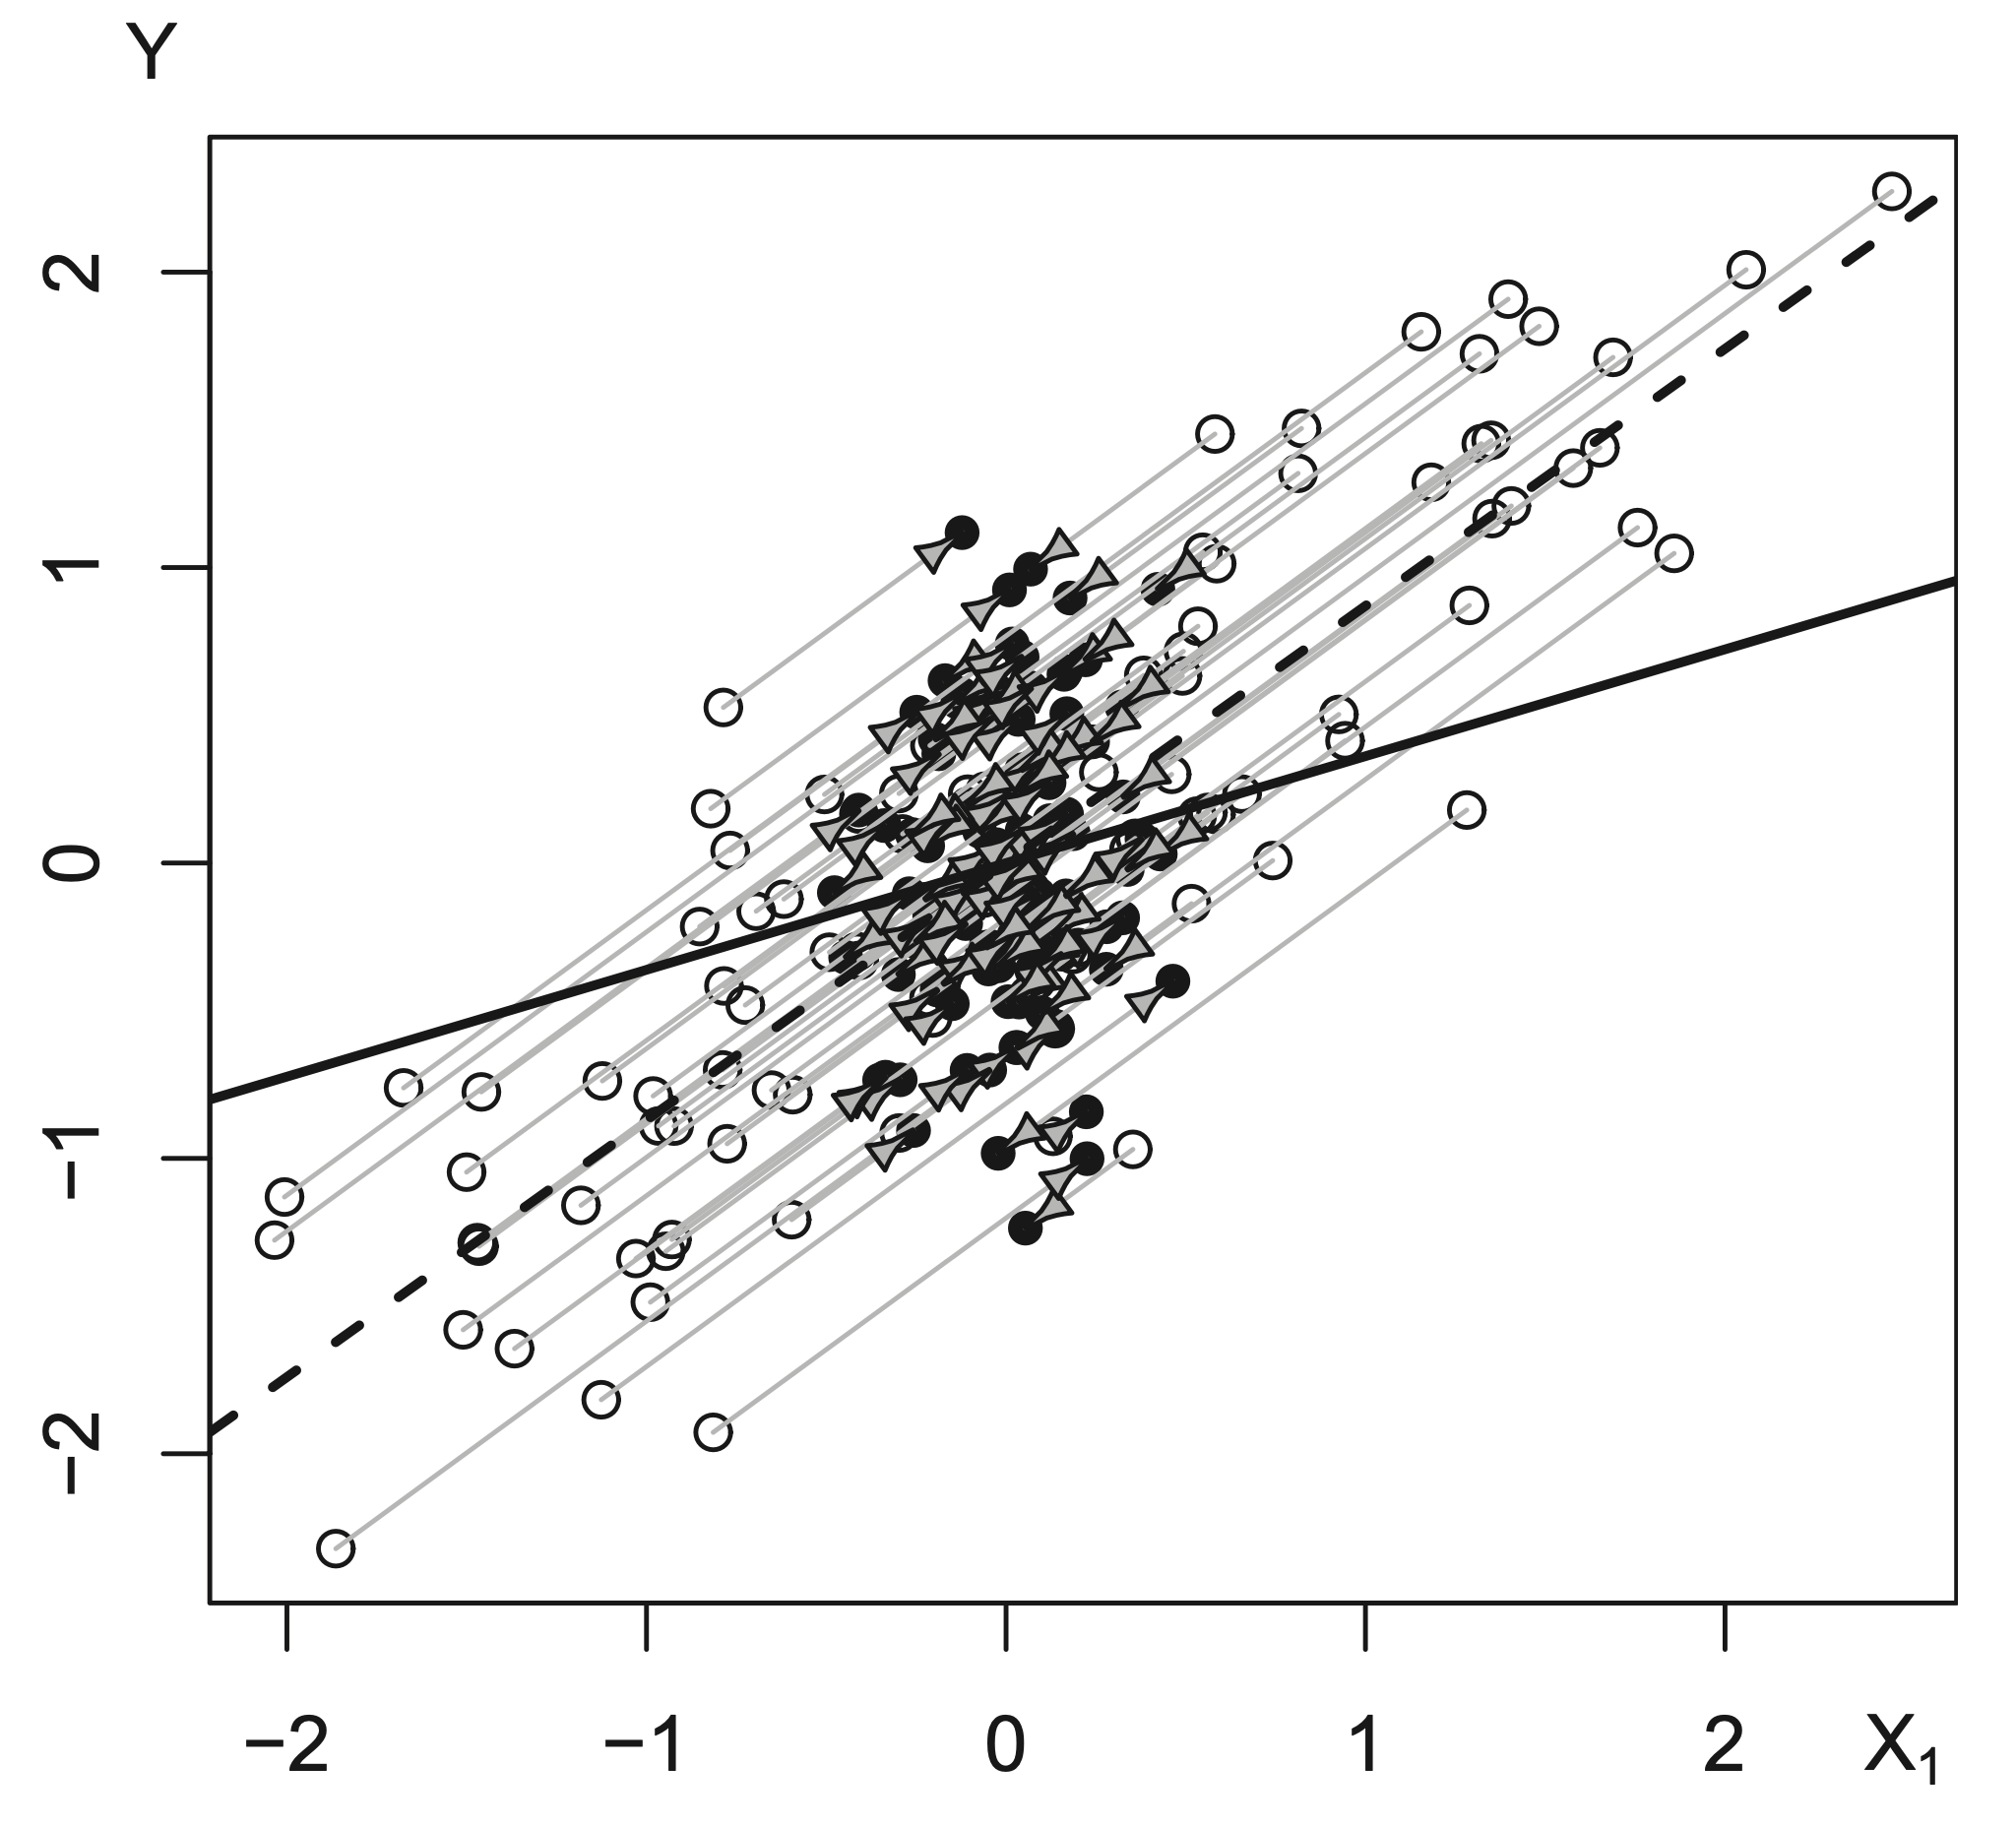
\includegraphics[width=0.9\textwidth]{Lecture17/JF_11_9}
  \caption{
  The marginal scatterplot (open circles) for $Y$ and $X_1$ superimposed on the added-variable plot (filled circles) for $X_1$ in the regression of $Y$ on $X_1$ and $X_2$.
  The variables $Y$ and $X_1$ are centered at their means to facilitate the comparison of the two sets of points.
  The arrows show how the points in the marginal scatterplot map into those in the AV plot.
  In this contrived data set, $X_1$ and $X_2$ are highly correlated ($r_{12} = 0.98$), and so the conditional variation in $X_1$ (represented by the horizontal spread of the filled points) is much less than its marginal variation (represented by the horizontal spread of the open points).
  The broken line gives the slope of the marginal regression of $Y$ on $X_1$ alone, while the solid line gives the slope $\hat{\beta}_1$ of $X_1$ in the MLR of $Y$ on both $X$s.
   JF Figure 11.9.}
  \label{fig:avp}
\end{center}
\end{figure}
%

Figure~\ref{fig:duncan_avp} illustrates the added-variable plots using the Duncan's data.
%
\begin{figure}[H]
\begin{center}
  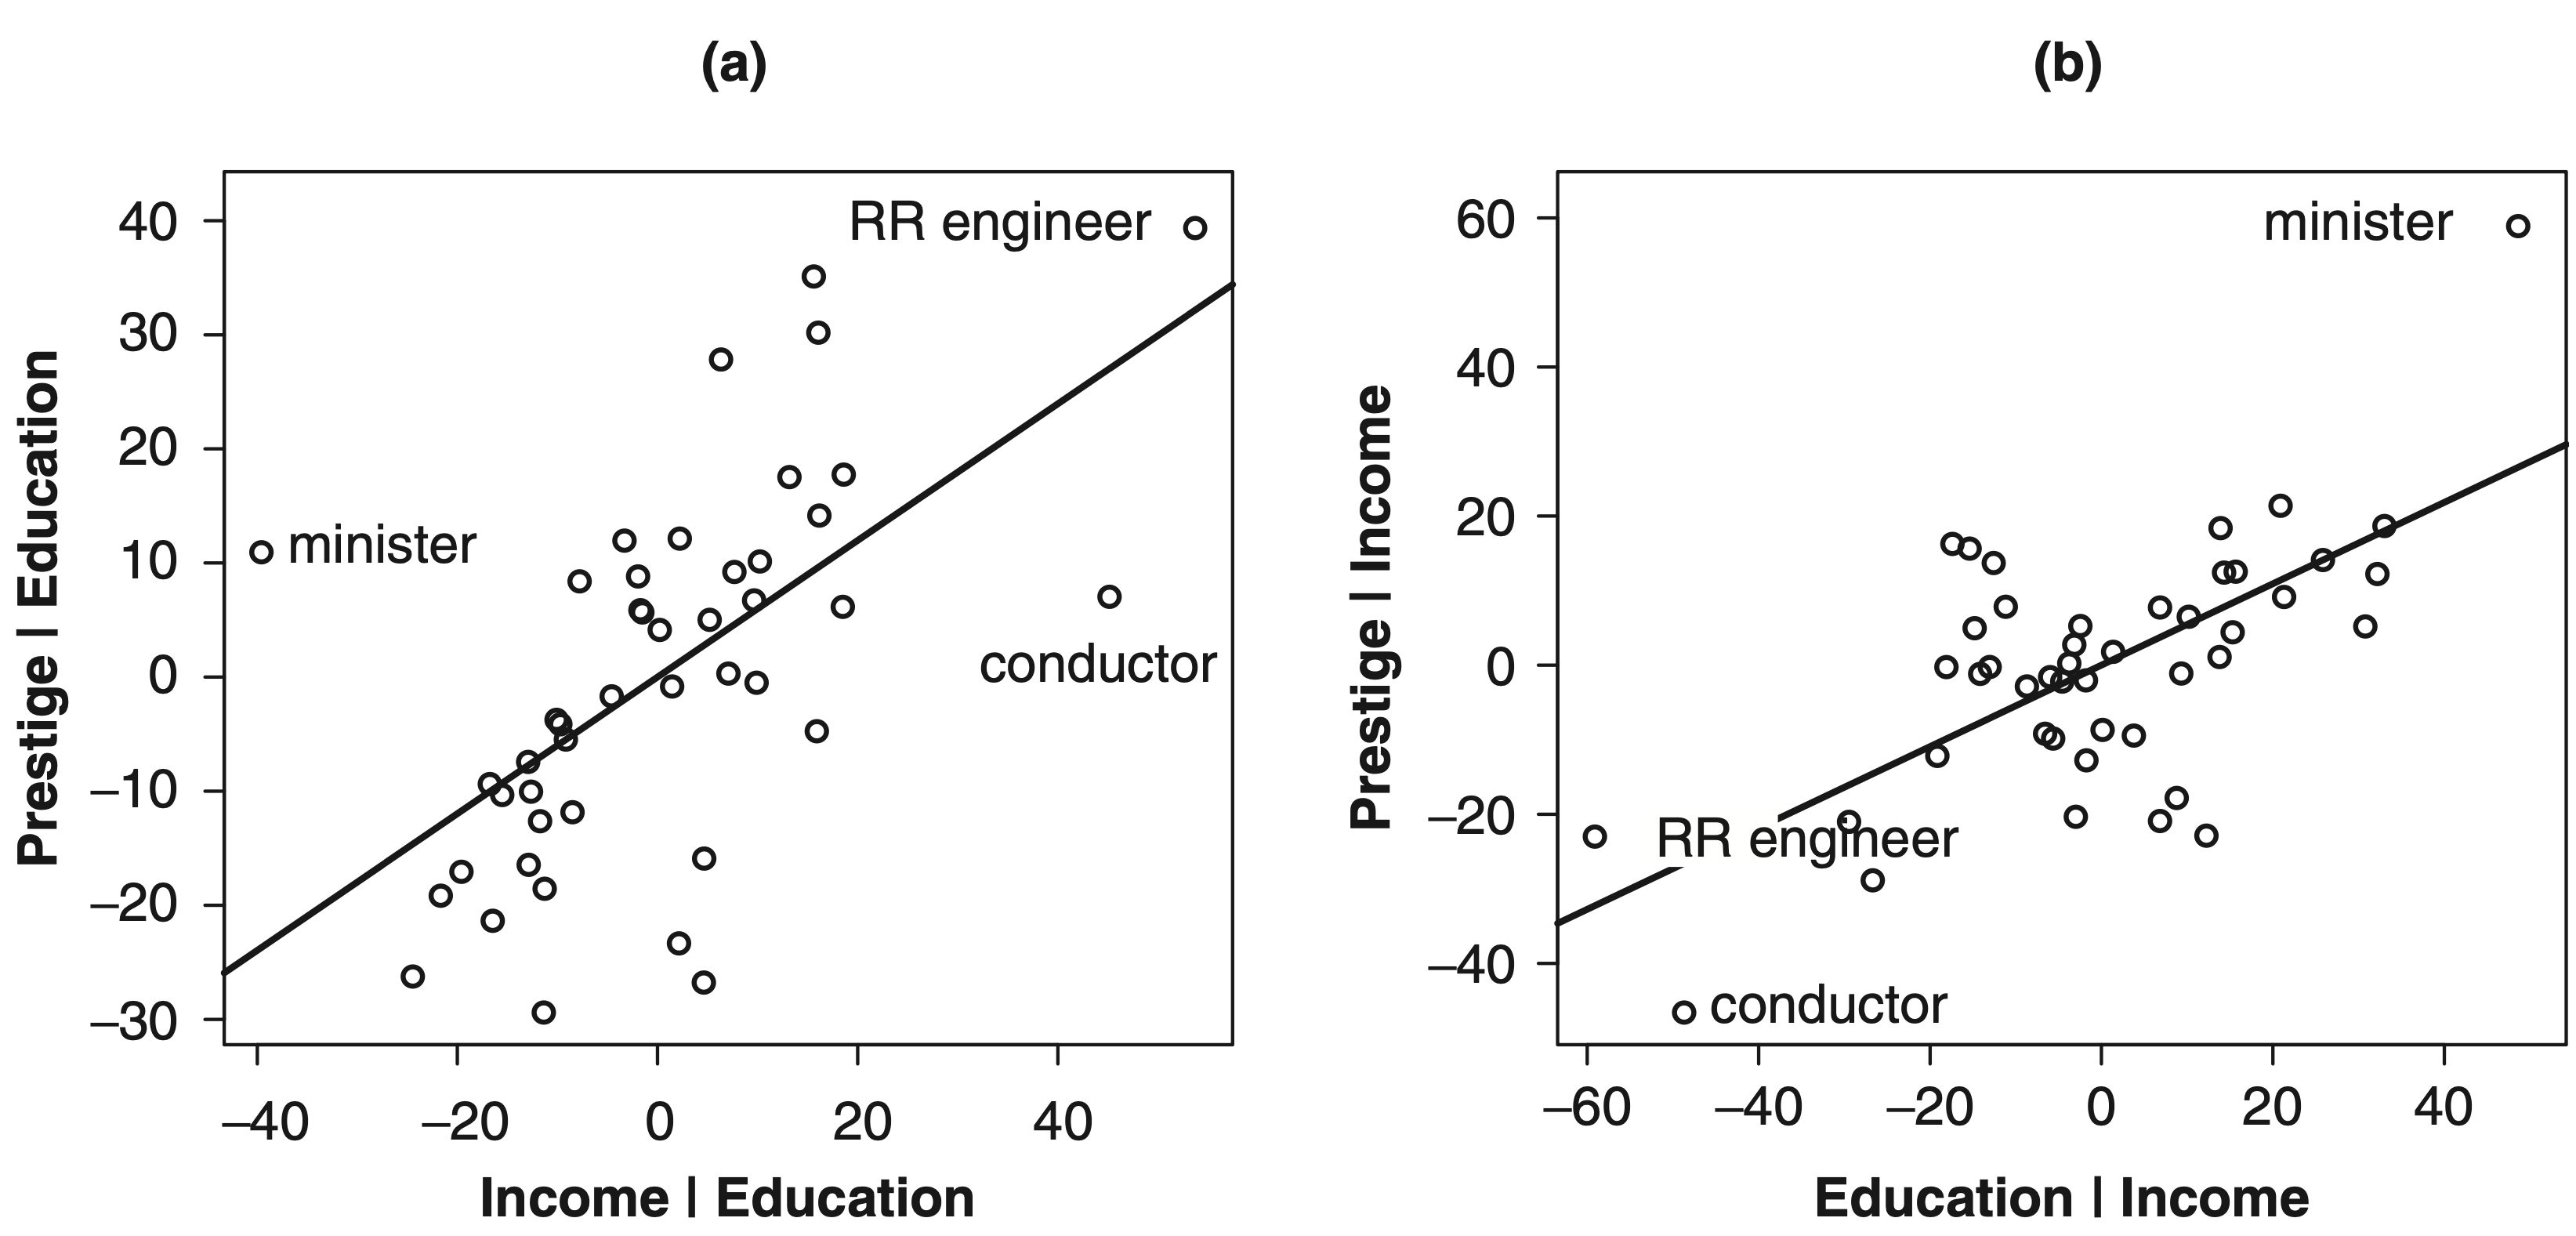
\includegraphics[width=0.9\textwidth]{Lecture17/JF_11_10}
  \caption{
  Added-variable plots for Duncan's regression of occupational prestige on the (a) income and (b) education levels of 45 US occupations in 1950.
  Three unusal observations, $miniters$, $conductors$, and $railroad engineers$, are identified on the plots.
  The added-variable plot for the intercept $\hat{\beta}_0$ is not shown.
   JF Figure 11.10.}
  \label{fig:duncan_avp}
\end{center}
\end{figure}
%

\subsection*{Should unusual data be discarded?}
In practice, although problematic data should not be ignored, they also should not be deleted automatically and without reflection:
\begin{itemize}
  \item It is important to investigate {\it why} an observation is unusual.  Truly ``bad'' data (e.g., an error in data entry ) can often be corrected or, if correction is not possible, thrown away.
  When a discrepant data point is correct, we may be able to understand why the observation is unusual.  
  For Duncan's data, for example, it makes sense that ministers enjoy prestige not accounted for by the income and educational levels of the occupation and for a reason not shared by other occupations.
  In a case like this, where an outlying observation has characteristics that render it unique, we may choose to set it aside from the rest of the data.
  \item Alternatively, outliers, high-leverage points, or influential data may motivate model respecification, and the pattern of unusual data may suggest the introduction of additional explanatory variables.
  We noticed, for example, that both conductors and railroad engineers had high leverage in Duncan's regression because these occupations combined relatively high income with relatively low education.
  Perhaps this combination of characteristics is due to a high level of unionization of these occupations in 1950, when the data were collected.
  If so, and if we can ascertain the levels of unionization of all of the occupations, we could enter this as an explanatory variable, perhaps shedding further light on the process determining occupational prestige.
  \item Except in clear-cut cases, we are justifiably reluctant to delete observations or to respecify the model to accommodate unusual data.
  Some researchers reasonably adopt alternative estimation strategies, such as robust regression, which continuously downweights outlying data rather than simply discarding them.
  Because these methods assign zero or very small weight to highly discrepant data, however, the result is generally not very different from careful application of least squares, and , indeed, robust-regression weights can be used to identify outliers.
  \item Finally, in large samples, unusual data substantially alter the results only in extreme instances.
  Identifying unusual observations in a large sample, therefore, should be regarded more as an opportunity to learn something about the data not captured by the model that we have fit, rather than as an occasion to reestimate the model with the unusual observations removed.
  
\end{itemize}



